% Traceability: derived from supplement-c/examples/07_c7_brownian_bacteria_motion.tex
\subsection{Biological systems}

\subsubsection{Brownian bacteria ominion witness}
\label{man:brownian-bacteria-witness}
\colabbadge{manual/notebooks/04d_biological_bacteria.ipynb}

\begin{table}[H]
\centering
\caption{Bacteria retained-extraction declaration.}
\label{tab:bacteria-retention}
\begin{threeparttable}
\begin{tabularx}{\linewidth}{@{}lX@{}}
\toprule
Item & Declaration \\
\midrule
Parent field & cited biological AO field \\
Retained extraction & bacteria ominion jitter field \\
Omitted context & environmental and colony-scale contexts outside the cited window \\
First refinement & longer-window biological drift ledger \\
Validity window & cited bacteria window \\
Residual witness & qualitative until refinement row is computed \\
\bottomrule
\end{tabularx}
\end{threeparttable}
\end{table}

A cited bacteria window is fixed first and then carried into the mass-scaled loss/tension, cadence-noise, and drift witnesses.

\begin{table}[H]
\centering
\caption{Bacteria ominion cited row.}
\label{tab:bacteria-ominion-row}
\begin{threeparttable}
\small
\begin{tabularx}{\linewidth}{@{}lXccc@{}}
\toprule
Row & Structural key & $B^*$ & $\Lambda_b$ & $R_{\mathrm{loss}}$ [\(\mathrm{trit}/\mathrm{bip}_0\)] \\
\midrule
B1 & \texttt{tetron:*:[bacteria]:6} & 2 & 11 & mass-scaled service burden \\
\bottomrule
\end{tabularx}
\ManualTableNote{The cited bacteria window carries a mass-scaled loss/tension burden together with a cadence-noise band and a recurrent drift witness on one ledger.}
\end{threeparttable}
\end{table}

\begin{figure}[H]
\centering
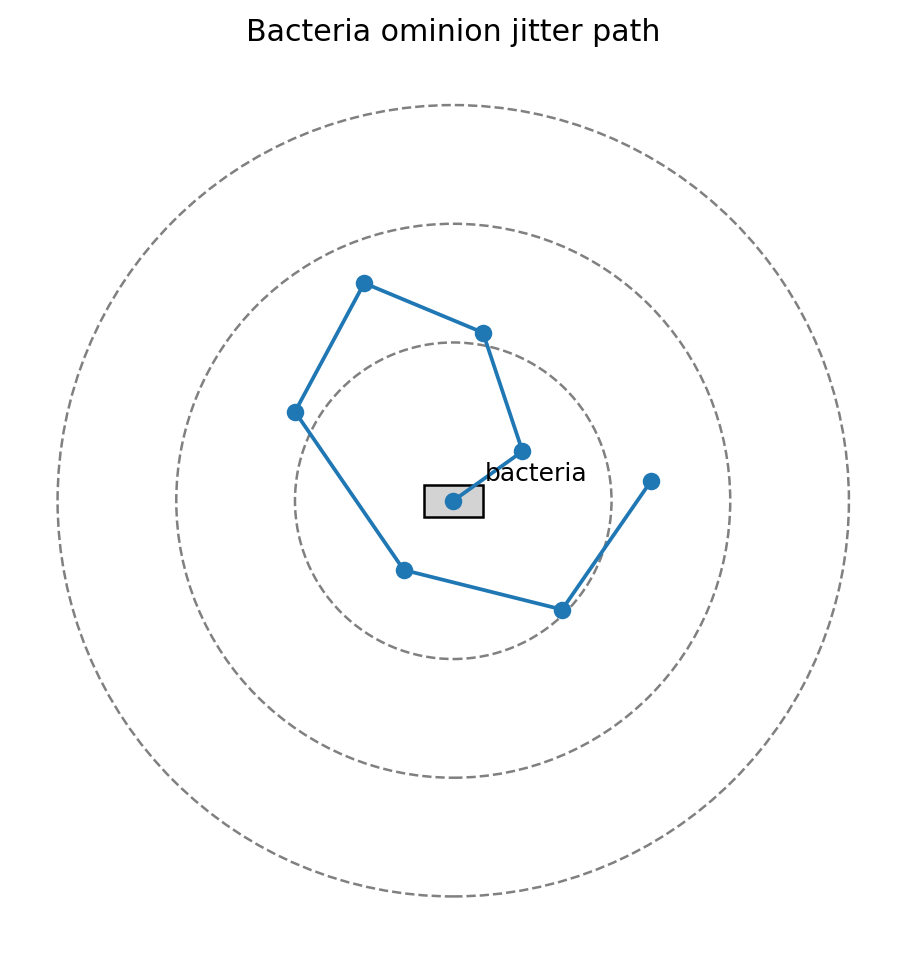
\includegraphics[width=0.66\linewidth]{figures/bacteria/01_bacteria_ominion.png}
\caption{Bacteria ominion jitter path with shell-like dwell bands.}
\label{fig:bacteria-ominion}
\end{figure}

The cited bacteria ledger carries the recurrent-jitter and dwell-distribution witnesses on the same window.
